\subsection{Hidden Markov Models}
\label{sec:hmmExperiments-sachin}

Having examined briefly the theory behind Hidden Markov Models, let us now look at how the training was done offline, and analyse some results from subsequent tests. As mentioned earlier, the apnoeatic states are modelled as the hidden states $\{x_t\}_1^T$, and are elements of the binary set $\{0, 1\}$. The observed signal is annotated every K samples (every minute in the case of the PhysioNet data), so we stack all K samples into $\vec y_t \in \mathbb{R}^d$, ($d = K$). Using the packages \verb!pmtk3! and \verb!HMM Toolbox!, the algorithms were implemented in \verb!MATLAB!\textsuperscript{\textregistered}, along with the conditioning of the data using spectrogram and PCA analysis. Again, \verb!MATLAB!\textsuperscript{\textregistered} is used for convenience and the code can be easily converted to \verb!Java! after experimentation and analysis.

The data is read and conditioned as explained in Section \ref{sec:RandCDatainMATLAB}.

We then move on to training and fitting the parameters, using the \verb!pmtk3! and \verb!HMM Toolbox! packages. We then compare the expected hidden states calculated using the \verb!Viterbi Algorithm! with the actual underlying states and determine the accuracy of the HMM model diagnosis.

The parameters are fitted using the \verb!apneaHMMTrain! function shown in Appendix \ref{sec:apneaHMMTrain}, which computes the transitional matrix \verb!A! using

\begin{align}
		A_{ij} & = \frac{\sum_{t = 1}^{T - 1} 1\{x_t = s_i \land x_{t + 1} = s_j\}}{\sum_{t = 1}^{T} 1\{x_t = s_i\}}
\end{align}

and uses Gaussian fitting to calculate the pdfs for the emissions (the \verb!gaussFit! function is used from the \verb!HMM Toolbox! package -- we shall not go into the details on how the function is implemented here). We are left with the outputs \verb!A!, the 2x2 transition matrix, \verb!Mu! and \verb!U!, parameters of the Gaussian pdf fit of the emissions, and \verb!pi!, the initial state distribution.

In order to compare with the test data, we need to read the data specified using \verb!testIndex!, condition it, and use the \verb!Viterbi Algorithm! to calculate the most likely path. This is done in the function \verb!apneaHMMTest!, found in Appendix \ref{sec:apneaHMMTest}. The code for reading and conditioning the data (and plotting the results) has been ommitted as it is similar to that shown before. Once again, functions from `off-the-shelf' packages are used in implementing the \verb!Viterbi Algorithm! and the accuracy of the most likely path is calculated by comparing it to the annotations reflecting the true states. This is done for each test file, and the results are shown below, in Figure \ref{fig:hmmExperiment}.

\begin{figure}[ht]
		\centering
		\subfloat[record 11]{%
			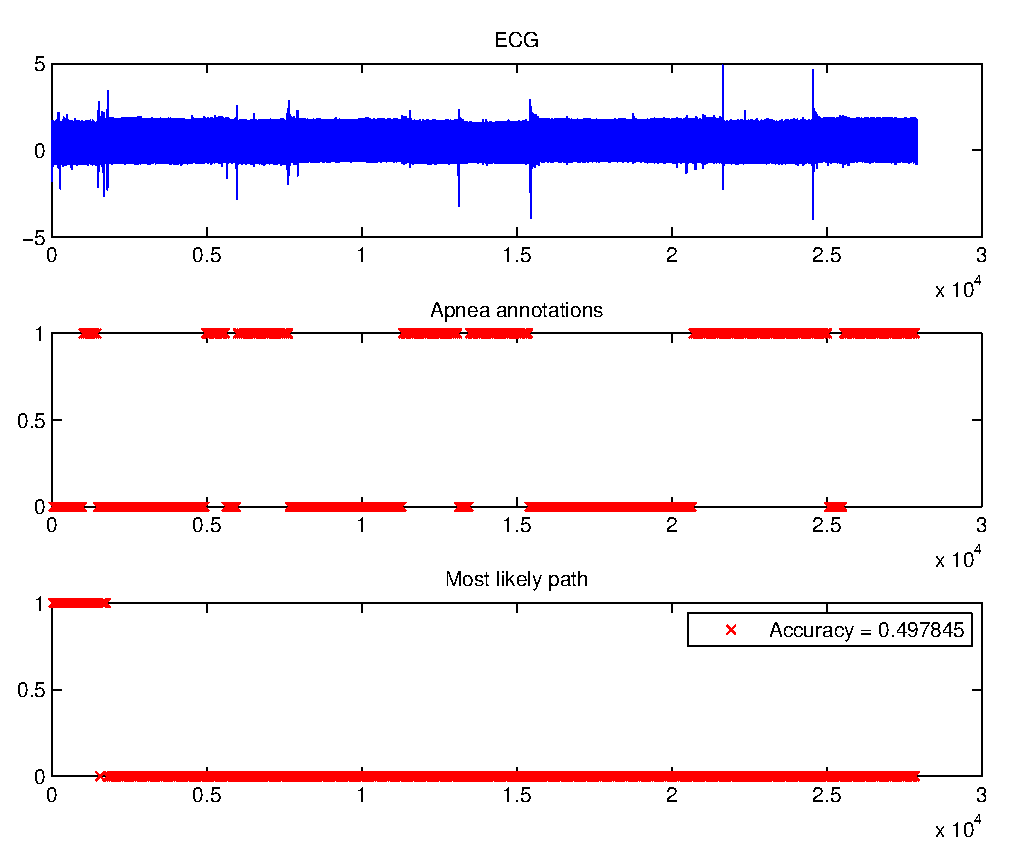
\includegraphics[width=.33\textwidth]{drawings/hmm/hmmTest11}}
		\subfloat[record 12]{%
			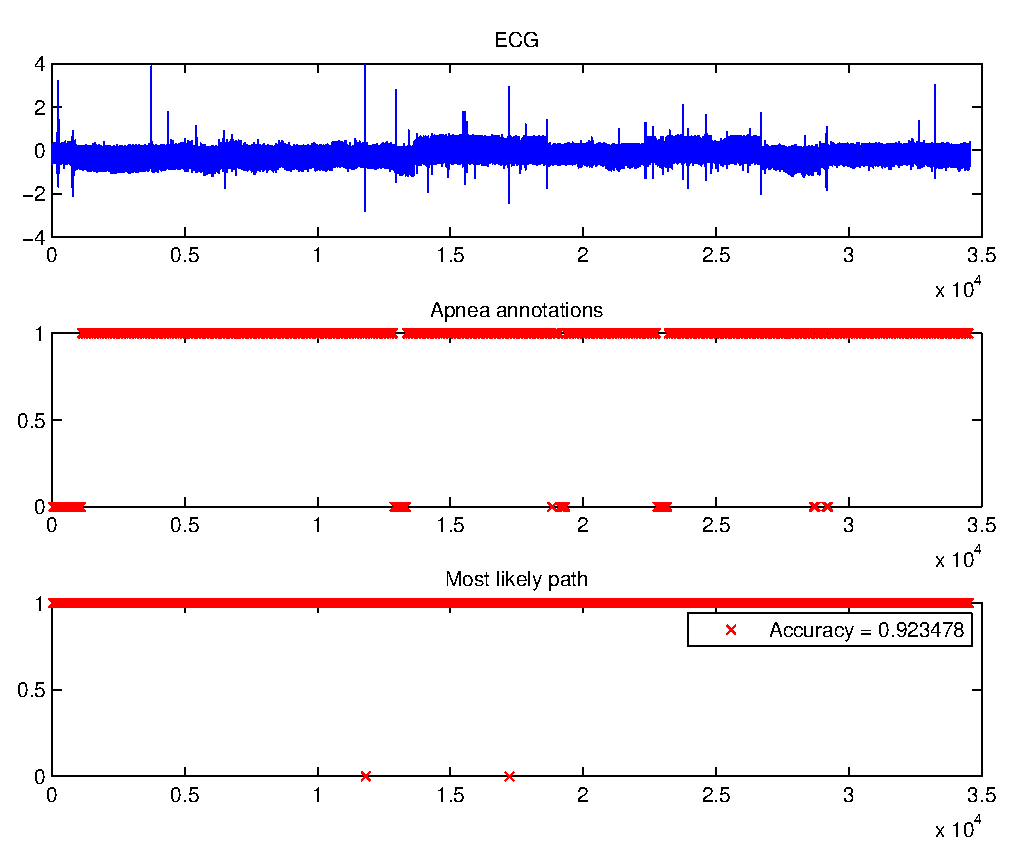
\includegraphics[width=.33\textwidth]{drawings/hmm/hmmTest12}}
		\subfloat[record 13]{%
			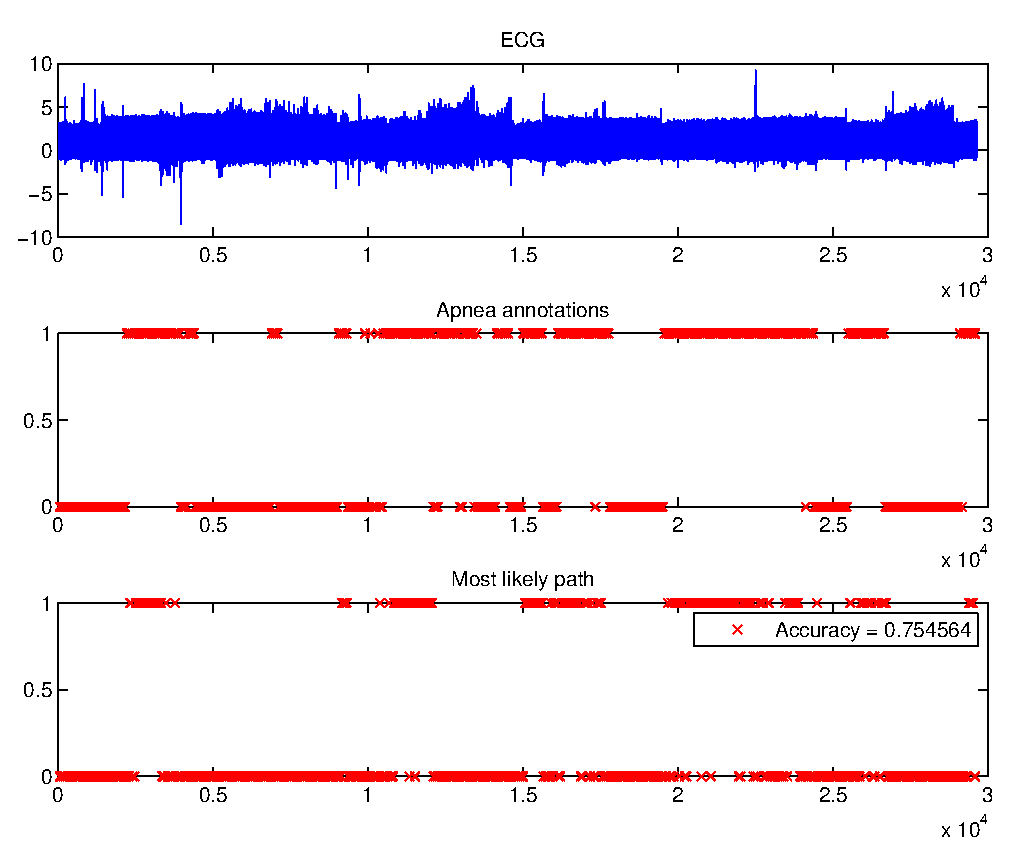
\includegraphics[width=.33\textwidth]{drawings/hmm/hmmTest13}} \\
		\subfloat[record 14]{%
			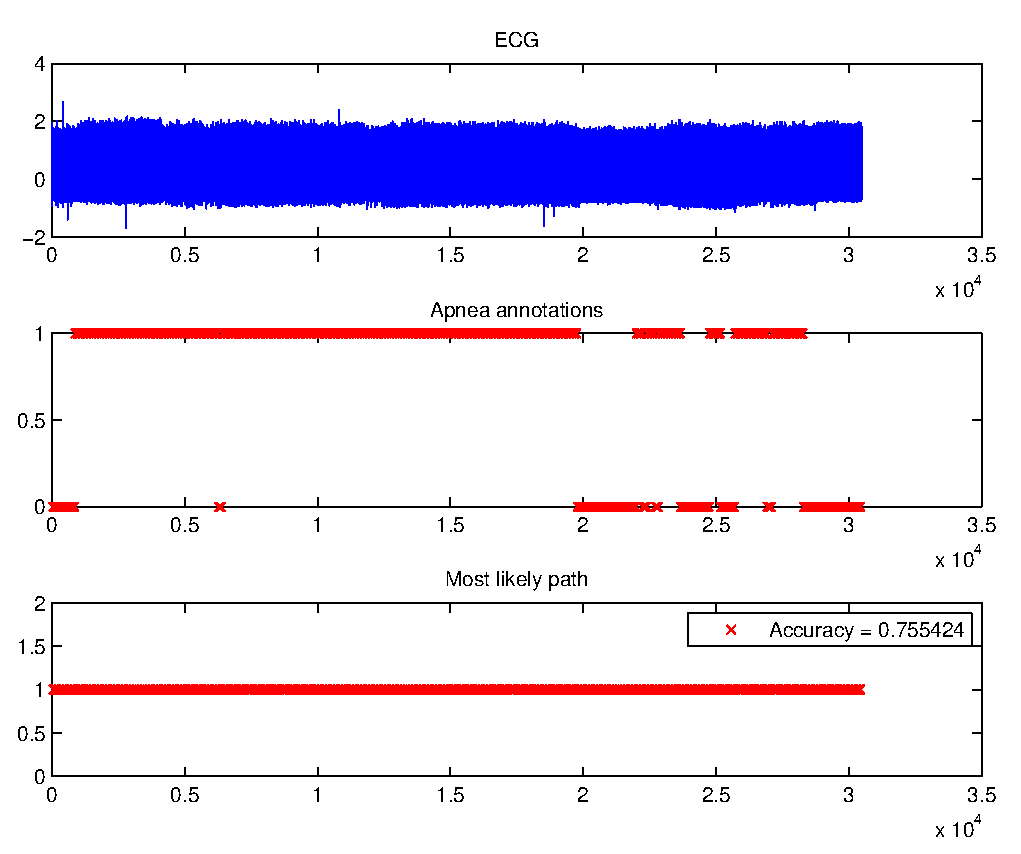
\includegraphics[width=.33\textwidth]{drawings/hmm/hmmTest14}}
		\subfloat[record 15]{%
			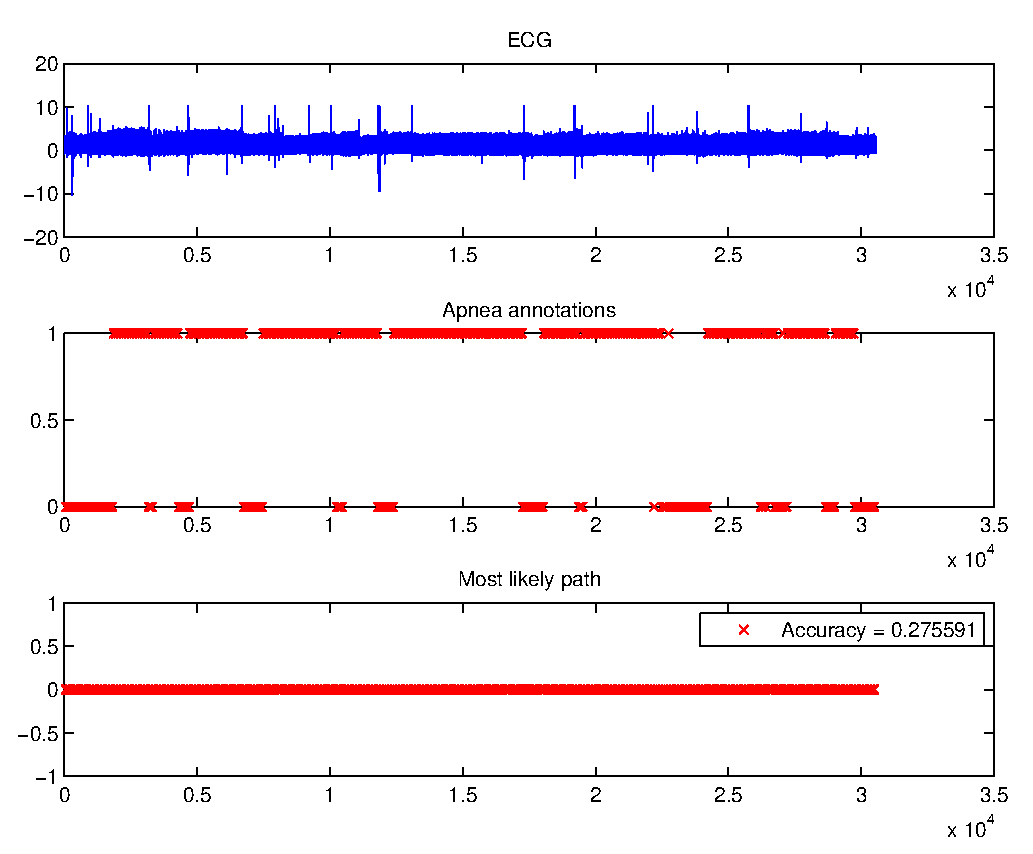
\includegraphics[width=.33\textwidth]{drawings/hmm/hmmTest15}}
		\caption{Performance of HMM model on the test records 11 to 15}
		\label{fig:hmmExperiment}
\end{figure}
